% =============================================================================
%  The assumptions of a one-dimensional PBL closure, as a pyramid (standalone)
%  Companion to pbl_assumptions_table.tex (rows A1-C10 = Table I.1; D3-D8 added here).
%  Build: source ~/miniconda3/bin/activate tex && tectonic pbl_assumptions_pyramid.tex
%  Layout rule: a block touches at its bottom exactly the blocks it relies on; blocks
%  on one level never touch (air gap 0.10 cm). Unit width 1.22 cm, doubles 2.54 cm,
%  level 1 starts at x = 0.6 so the ground sticks out on both sides. Two levels above
%  the ground, no top row (2026-09-16 evening: D8 folded into A2, C3 and D7 into C2).
%  Ground order is forced by the adjacency chain GAP-HOM-STA-SIM-ISOb-AXI-BOU: B6 is
%  split into the constant-flux layer (HOM+STA) and Monin-Obukhov similarity (STA+SIM),
%  which is what puts similarity under MOST; the AXI/BOU boundary sits under the left
%  part of C8 so that BOU has room for its text.
% =============================================================================
\documentclass[10pt]{article}
\usepackage{iftex}
\ifPDFTeX
  \usepackage[utf8]{inputenc}
  \usepackage[T1]{fontenc}
  \usepackage{lmodern}
\else
  \usepackage{fontspec}
  \setmainfont{lmroman10-regular.otf}[BoldFont=lmroman10-bold.otf,
    ItalicFont=lmroman10-italic.otf, BoldItalicFont=lmroman10-bolditalic.otf]
\fi
\usepackage[british]{babel}
\usepackage[a4paper,landscape,margin=10mm,top=9mm,bottom=9mm]{geometry}
\usepackage{amsmath,amssymb}
\usepackage{xcolor}
\usepackage{tikz}
\usepackage{microtype}
\pagestyle{empty}
\setlength{\parindent}{0pt}
\setlength{\parskip}{0.5ex}

% ---- notation ---------------------------------------------------------------
\newcommand{\avg}[1]{\langle #1 \rangle}
\newcommand{\pd}[2]{\partial #1/\partial #2}
\newcommand{\qsq}{q^{2}}
\newcommand{\Rfc}{R_{fc}}
\newcommand{\dx}{\Delta x}
% ---- rows the PhD concept turns on (same data as the note's macros.tex) ------
\definecolor{cKey}{HTML}{7B2D8E}
\newcommand{\setkey}[2]{\expandafter\def\csname key@#1\endcsname{#2}}
\makeatletter
\setkey{A1}{1}\setkey{B1}{1}\setkey{B2}{1}\setkey{B3}{1}\setkey{C3}{1}\setkey{C4}{1}\setkey{C6}{1}\setkey{C7}{1}
\setkey{B5}{2}\setkey{B6}{2}\setkey{C2}{2}\setkey{C5}{2}\setkey{C9}{2}
\newcommand{\keymark}[1]{\ifcsname key@#1\endcsname
  \if1\csname key@#1\endcsname\textcolor{cKey}{$\blacktriangleright$}\else\textcolor{cKey}{$\triangleright$}\fi\fi}
\makeatother
\newcommand{\pid}[1]{\keymark{#1}\textbf{#1}}
% \pb{x0}{x1}{y0}{y1}{style}{text}: a block from (x0,y0) to (x1,y1), text centred
\newcommand{\pb}[6]{\pgfmathsetmacro{\pbw}{#2-#1-0.20}%
  \draw[#5] (#1,#3) rectangle (#2,#4);
  \node[align=center, font=\tiny, inner sep=0pt, text width=\pbw cm] at ({(#1+#2)/2},{(#3+#4)/2}) {#6};}

\begin{document}
{\Large\bfseries The assumptions of a one-dimensional PBL closure, as a pyramid: what rests on what}\\[0.3ex]
{\small Companion to the assumptions note (rows A1--C10 are its Table~I.1; D3--D6 are added here). 2026-09-16.}

\vspace{0.6ex}
{\footnotesize Every block is an assumption a boundary-layer scheme makes in order to run. A block touches at its
bottom exactly the blocks it relies on, and blocks on one level do not touch each other. Dark grey: the ground ---
seven hypotheses that rest on nothing else here. Light grey: hypotheses that themselves presuppose another
(the Reynolds conditions and locality presuppose the gap; ergodicity in space presupposes homogeneity across the
cell, its second premise --- many decorrelated eddies per cell --- being A1's contact on A2; the scalar eddy
viscosity is Rotta's isotropy evaluated with one axis). White: the closure's assumptions, with the concept marks
of the note ($\blacktriangleright$ a research question turns on it, $\triangleright$ the project's methods do).
Each block shows its primary reliance; the incidence matrix of the note has the full set. Not drawn, because no
scheme needs them to run: ergodicity in time and Taylor's hypothesis, which carry the observations and the
calibration; the constraints realizability and Galilean invariance, which bound the algebra rather than carry a
block; and the dynamical core's numerical dissipation. The fixed reference temperature of the buoyancy coefficient
sits inside the Boussinesq block.\par}

\vspace{1.2ex}
\begin{center}
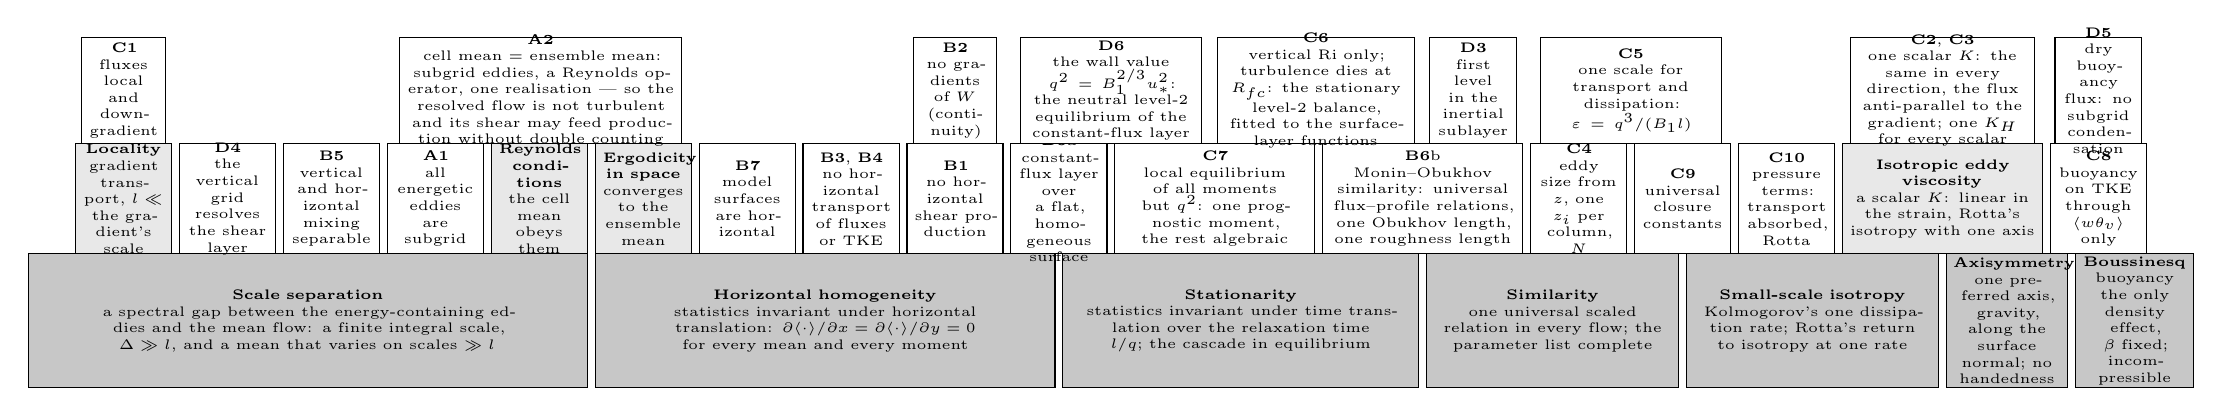
\begin{tikzpicture}[x=1cm, y=1cm,
  ground/.style={draw, line width=0.4pt, fill=black!22},
  hyp/.style={draw, line width=0.4pt, fill=black!9},
  row/.style={draw, line width=0.4pt, fill=white}]
% ---- level 0: the ground (y 0 -- 1.7); each boundary sits under the block that spans it -----------
\pb{0}{7.10}{0}{1.7}{ground}{\textbf{Scale separation}\\ a spectral gap between the energy-containing eddies and the mean flow: a finite integral scale, \mbox{$\Delta \gg l$}, and a mean that varies on scales \mbox{$\gg l$}}
\pb{7.20}{13.04}{0}{1.7}{ground}{\textbf{Horizontal homogeneity}\\ statistics invariant under horizontal translation: \mbox{$\pd{\avg{\cdot}}{x} = \pd{\avg{\cdot}}{y} = 0$} for every mean and every moment}
\pb{13.14}{17.66}{0}{1.7}{ground}{\textbf{Stationarity}\\ statistics invariant under time translation over the relaxation time $l/q$; the cascade in equilibrium}
\pb{17.76}{20.96}{0}{1.7}{ground}{\textbf{Similarity}\\ one universal scaled relation in every flow; the parameter list complete}
\pb{21.06}{24.26}{0}{1.7}{ground}{\textbf{Small-scale isotropy}\\ Kolmogorov's one dissipation rate; Rotta's return to isotropy at one rate}
\pb{24.36}{25.90}{0}{1.7}{ground}{\textbf{Axisymmetry}\\ one preferred axis, gravity, along the surface normal; no handedness}
\pb{26.00}{27.50}{0}{1.7}{ground}{\textbf{Boussinesq}\\ buoyancy the only density effect, $\beta$ fixed; incompressible}
% ---- level 1 (y 1.7 -- 3.1): 14 single blocks of 1.22 cm, 3 doubles of 2.54 cm, air gap 0.10 -----
\pb{0.60}{1.82}{1.7}{3.1}{hyp}{\textbf{Locality}\\ gradient transport, $l \ll$ the gradient's scale}
\pb{1.92}{3.14}{1.7}{3.1}{row}{\textbf{D4}\\ the vertical grid resolves the shear layer}
\pb{3.24}{4.46}{1.7}{3.1}{row}{\pid{B5}\\ vertical and horizontal mixing separable}
\pb{4.56}{5.78}{1.7}{3.1}{row}{\pid{A1}\\ all energetic eddies are subgrid}
\pb{5.88}{7.10}{1.7}{3.1}{hyp}{\textbf{Reynolds conditions}\\ the cell mean obeys them}
\pb{7.20}{8.42}{1.7}{3.1}{hyp}{\textbf{Ergodicity in space}\\ converges to the ensemble mean}
\pb{8.52}{9.74}{1.7}{3.1}{row}{\pid{B7}\\ model surfaces are horizontal}
\pb{9.84}{11.06}{1.7}{3.1}{row}{\pid{B3}, \textbf{B4}\\ no horizontal transport of fluxes or TKE}
\pb{11.16}{12.38}{1.7}{3.1}{row}{\pid{B1}\\ no horizontal shear production}
\pb{12.48}{13.70}{1.7}{3.1}{row}{\pid{B6}a\\ constant-flux layer over a flat, homogeneous surface}
\pb{13.80}{16.34}{1.7}{3.1}{row}{\pid{C7}\\ local equilibrium of all moments but $\qsq$: one prognostic moment, the rest algebraic}
\pb{16.44}{18.98}{1.7}{3.1}{row}{\pid{B6}b\\ Monin--Obukhov similarity: universal flux--profile relations, one Obukhov length, one roughness length}
\pb{19.08}{20.30}{1.7}{3.1}{row}{\pid{C4}\\ eddy size from $z$, one $z_i$ per column, $N$}
\pb{20.40}{21.62}{1.7}{3.1}{row}{\pid{C9}\\ universal closure constants}
\pb{21.72}{22.94}{1.7}{3.1}{row}{\textbf{C10}\\ pressure terms: transport absorbed, Rotta}
\pb{23.04}{25.58}{1.7}{3.1}{hyp}{\textbf{Isotropic eddy viscosity}\\ a scalar $K$: linear in the strain, Rotta's isotropy with one axis}
\pb{25.68}{26.90}{1.7}{3.1}{row}{\textbf{C8}\\ buoyancy on TKE through $\avg{w\theta_v}$ only}
% ---- level 2 (y 3.1 -- 4.45): the top of the closure -------------------------------------------------
\pb{0.68}{1.74}{3.1}{4.45}{row}{\textbf{C1}\\ fluxes local and down-gradient}
\pb{4.72}{8.30}{3.1}{4.45}{row}{\textbf{A2}\\ cell mean $=$ ensemble mean: subgrid eddies, a Reynolds operator, one realisation --- so the resolved flow is not turbulent and its shear may feed production without double counting}
\pb{11.24}{12.30}{3.1}{4.45}{row}{\pid{B2}\\ no gradients of $W$ (continuity)}
\pb{12.60}{14.90}{3.1}{4.45}{row}{\textbf{D6}\\ the wall value $\qsq = B_1^{2/3} u_*^2$: the neutral level-2 equilibrium of the constant-flux layer}
\pb{15.10}{17.60}{3.1}{4.45}{row}{\pid{C6}\\ vertical Ri only; turbulence dies at $\Rfc$: the stationary level-2 balance, fitted to the surface-layer functions}
\pb{17.80}{18.90}{3.1}{4.45}{row}{\textbf{D3}\\ first level in the inertial sublayer}
\pb{19.20}{21.50}{3.1}{4.45}{row}{\pid{C5}\\ one scale for transport and dissipation: $\varepsilon = q^3/(B_1 l)$}
\pb{23.14}{25.48}{3.1}{4.45}{row}{\pid{C2}, \pid{C3}\\ one scalar $K$: the same in every direction, the flux anti-parallel to the gradient; one $K_H$ for every scalar}
\pb{25.74}{26.84}{3.1}{4.45}{row}{\textbf{D5}\\ dry buoyancy flux: no subgrid condensation}
\end{tikzpicture}
\end{center}

\vspace{0.8ex}
{\footnotesize\textbf{Reading.} Two levels stand on the ground. On the left, the grey zone: the gap makes the eddies
subgrid (A1), the operator and the ergodic premise make the cell mean an ensemble mean (A2), and only then may the
model's own gradients feed production as ensemble gradients --- the clause of A2 that fails first when the grid
resolves part of the spectrum. In the middle, the surface: the note's B6 is two blocks here, because Monin--Obukhov
similarity rests on similarity as much as on the constant-flux layer and one block cannot touch three foundations
without covering the middle one --- so the constant-flux layer (B6a) rests on homogeneity and stationarity, and
Monin--Obukhov similarity (B6b) rests on stationarity and similarity. On the pair rest the wall value of $\qsq$
(D6, from the constant-flux layer and local equilibrium), the placement of the first level (D3, from similarity's
domain of validity) and the Richardson cutoff (C6, from the stationary level-2 balance whose functions were fitted
to the surface-layer functions and inherit their critical Richardson number). On the right, the tensor: a linear
isotropic eddy viscosity gives one scalar $K$, the same in every direction, aligned with the gradient and shared
by every scalar (C2 with C3); one master length carries both transport and dissipation (C5); the one-axis
buoyancy term of a Boussinesq fluid (C8) carries the dry buoyancy flux (D5). The middle carries the night, the
left the convective day, the right the closure of the tensor.\par}

\vspace{0.6ex}
{\footnotesize\textbf{Changes against the note's rows.} B6 split into B6a (constant-flux layer) and B6b
(Monin--Obukhov similarity). B3 and B4 one block: no horizontal transport of fluxes or of TKE. C3 folded into C2:
one scalar $K$ is one assumption seen twice, and the mixing of all scalars alike is its third face. Added: D3 the
first model level above the roughness sublayer and below any wind maximum ($z_0 \ll z_1 \ll z_i$); D4 the
vertical grid resolves the layer that produces the turbulence, the vertical counterpart of A1 with the sign
reversed; D5 the buoyancy flux of unsaturated air, saturation acting through the resolved condensation only; D6
the lower boundary of the TKE equation, $\qsq = B_1^{2/3} u_*^2$ (every MYNN-family scheme; the 3D closure fork
runs without it). Folded into A2: the resolved flow carries no turbulence, so the grid-mean shear is the
ensemble-mean shear in $P_s$. Which scheme drops which block is Table~I.0 of the note.\par}
\end{document}
